\documentclass[compress]{beamer}
\usepackage[utf8]{inputenc}
\usepackage[francais]{babel}
\usepackage[T1]{fontenc}
\usepackage{amssymb}
\usepackage{amsmath}
\usepackage{amsfonts}
\usepackage[]{algorithm2e}
\usepackage{amssymb}
\usepackage{verbatim}
\usepackage{listings}
\usepackage{color}
\usepackage{graphicx}
\usetheme[navigation]{UMONS}

\author{Clément Tamines, Florent Delgrange}
\title{Statistiques multidimensionnelles}
\subtitle[\ldots]{Arbre de décisions (CART)}

\setbeamercovered{transparent} 
\setbeamertemplate{navigation symbols}{} 
\institute{UMONS\\Faculté des Sciences\\BA 3 Sciences Informatiques\\[2ex]
  
\includegraphics[height=4ex]{UMONS}\hspace{2em}%
  \raisebox{-1ex}{
\includegraphics[height=6ex]{UMONS_FS}}}
\date{Juin 2016} 
\definecolor{darkgreen}{rgb}{0.0, 0.2, 0.13}
\subject{Statistiques multidimensionnelles} 
\lstset{ %
  language=R,                     % the language of the code
  basicstyle=\footnotesize,       % the size of the fonts that are used for the code
  numbers=left,                   % where to put the line-numbers
  numberstyle=\tiny\color{gray},  % the style that is used for the line-numbers
  stepnumber=1,                   % the step between two line-numbers. If it's 1, each line
                                  % will be numbered
  numbersep=5pt,                  % how far the line-numbers are from the code
  backgroundcolor=\color{white},  % choose the background color. You must add \usepackage{color}
  showspaces=false,               % show spaces adding particular underscores
  showstringspaces=false,         % underline spaces within strings
  showtabs=false,                 % show tabs within strings adding particular underscores
  frame=single,                   % adds a frame around the code
  rulecolor=\color{black},        % if not set, the frame-color may be changed on line-breaks within not-black text (e.g. commens (green here))
  tabsize=2,                      % sets default tabsize to 2 spaces
  captionpos=b,                   % sets the caption-position to bottom
  breaklines=true,                % sets automatic line breaking
  breakatwhitespace=false,        % sets if automatic breaks should only happen at whitespace
  title=\lstname,                 % show the filename of files included with \lstinputlisting;
                                  % also try caption instead of title
  keywordstyle=\color{blue},      % keyword style
  commentstyle=\color{darkgreen},   % comment style
  stringstyle=\color{violet},      % string literal style
  escapeinside={\%*}{*)},         % if you want to add a comment within your code
  morekeywords={*,...}            % if you want to add more keywords to the set
} 

\begin{document}

\begin{frame}
\titlepage
\end{frame}

\begin{frame}
\tableofcontents
\end{frame}

\section{Description de CART}
\subsection{Introduction}
\begin{frame}
\frametitle{Introduction}
Un \textbf{arbre de décision} est un outil de classement de données, les répartissant selon des critères. C'est une méthode \textbf{d'apprentissage}.
\begin{enumerate}
\item Chaque élément du jeu de données correspond à un vecteur de valeurs.
\item Chaque nœud de l'arbre correspond à un test sur la valeur d'un des attributs.
\item Chaque donnée est répartie selon la valeur booléenne résultante.
\end{enumerate}
Dans ce sens, une branche de l'arbre correspond donc à une décision.
\end{frame}

\subsection{Algorithme de construction le l'arbre CART}
\begin{frame}
\frametitle{Comment l'arbre est-il construit ?}
L'impureté d'un échantillon, aussi appelée \textbf{index de Gini}, permet de calculer l'hétérogénéité de celui-ci \textit{(= degré de mélange)}. On calcule l'index Gini d'une classe $i$ comme suit :
\[Gini(p_i) = p_i (1 - p_i)\]
Plus la probabilité d'une classe $i$ est proche de 0.5, plus l'index est élevé.
\end{frame}

\begin{frame}
\frametitle{Calcul de l'impureté d'une classe x}
\lstinputlisting{Impurete.R}
Avec x, la classe dont on calcule l'impureté (vecteur). Si on prend le jeu de données Titanic (ptitanic) fourni avec R, on peut calculer l'impureté du facteur survived avec : \begin{verbatim}
> I(ptitanic\$survived)\\
$\begin{bmatrix}1\end{bmatrix} 0.4721383$ \end{verbatim}
\end{frame}

\begin{frame}
\frametitle{Comment l'arbre est-il construit ?}
Le but est tel que chaque nœud divise l'ensemble de données en deux sous ensemble les plus homogènes possibles.
Un test est donc associé à un nœud de telle sorte à \textbf{maximiser la réduction d'impureté}.\\
On veut donc maximiser $\Delta I$, tel que
\[ \Delta I = p(A)I(A) - p(A_L)I(A_L) - p(A_R)I(A_R)\]
où A est le nœud courant pour un certain test, $A_L$, $A_R$ sont les enfants de gauche et de droite et I(A) est l'impureté du nœud A pour ce test.
\end{frame}

\begin{frame}
\frametitle{Exemple sur le jeu de données Titanic fourni avec R}
\lstinputlisting{reduction_impurete.R}
Il s'agit de la valeur de réduction d'impureté de la variable sex. Cette valeur d'impureté est la valeur maximale que l'on obtient au premier nœud de l'arbre et c'est donc ce test qui sera choisi lors de la construction de l'arbre.
\end{frame}

\begin{frame}
\frametitle{Algorithme de construction de l'arbre}
\begin{algorithm}[H]
\SetKwData{Left}{left}\SetKwData{This}{this}\SetKwData{Up}{up}
\SetKwFunction{Union}{Union}\SetKwFunction{FindCompress}{FindCompress}
\SetKwInput{Entree}{Entr\'ees}
\SetKwInput{Sortie}{Sorties}
\SetKw{Retour}{retourner}
\SetKwFor{Pour}{pour}{faire}{finpour}
\SetKwFor{Tq}{tant que}{faire}{fintq}
\SetKwFor{PourCh}{pour chaque}{faire}{fait}
\SetKwFor{PourTous}{pour tout}{faire}{fait}
\SetKwRepeat{Repeter}{répéter}{jusqu’à}
\SetKwIF{Si}{SinonSi}{Sinon}{si}{alors}{sinon si}{sinon}{{fin si}}
\SetKwSwitch{Match}{Case}{Other}{match}{ : }{cas}{autre cas}{{fin cas}}{{fin match}}

\Entree{Un jeu de données}

$arbre$ $\leftarrow$ initialiser arbre vide \\
$noeud$ $\leftarrow$ arbre$_{racine}$ \\
\Repeter{plus de nœuds sans classes}{
	\Si{$noeud$ est terminal}{
		affecter une classe à $noeud$\\
	}
	\Sinon{
		Affecter un test à $noeud$ selon la perte d'impureté\\
		$noeud_{Gauche} \leftarrow$ créer sous arbre\\
		$noeud_{Droite} \leftarrow$ créer sous arbre\\
	}
	$noeud \leftarrow$ nœud suivant dans $arbre$\\
}
\Retour $arbre$
\BlankLine
\end{algorithm}
\end{frame}

\begin{frame}
Note : on dit qu'un nœud est terminal si 
\begin{enumerate}
\item toutes les valeurs satisfaisant le test du père sont dans la même classe.
\item il n'y a plus d'attributs à tester à ce niveau
\end{enumerate}

Grâce à un arbre construit d'une telle façon, nous pouvons prédire où se situeront de nouveaux éléments dans celui-ci simplement en le parcourant.
\end{frame}

\section{Implémentation dans R}

\begin{frame}
Nous allons maintenant expliquer comment créer et utilser un arbre de décision dans R.\\

Nous allons utiliser la librairie \textbf{rpart}, 
\end{frame}

\begin{frame}
Afin d'illustrer l'utilisation de \textbf{rpart}, nous utiliserons le jeu de données \textrm{ptitanic} inclus dans R.\\
Ce jeu de données contient une liste de passagers du Titanic et pour chaque passager il donne les informations suivantes :\\
\begin{itemize}
 \item Le sexe de la personne,
 \item son age,
 \item la classe dans laquelle il se trouvait (1ère, 2ème ou 3ème),
 \item le nombre de frères/sœurs et d'époux qui se trouvait dans le bateau,
 \item le nombre de parents/enfants qui se trouvait dans le bateau,
 \item une valeur disant si la personne a survécu ou non au naufrage.
\end{itemize}
\end{frame}
\begin{frame}
La fonctionr part s'utilise de la manière suivante: \\
\lstinputlisting{rpart.r}
Nous indiquons que nous voulons le résultat de \textrm{survived} en fonction de l'age et du sexe.
Le graphique suivant est alors produit. Nous avons utilisés les librairie \textbf{rattle} et \textbf{RColorBrewer} ainsi que la fonction \textbf{francyRPartPlot} pour 
créer des arbres plus lisibles que ceux de base fournis par la fonction \textbf{plot}.
\end{frame}
\begin{frame}
Nous obtenons le résultat suivant avec \textbf{prp} :
Nous avons comme information une condition sur la valeur d'une variable, les branches correspondantes respectant ou non cette condition.
Chaque noeud contient le nombre de personnes mortes et vivantes pour les choix effectués sur les variables.

      \begin{center}
            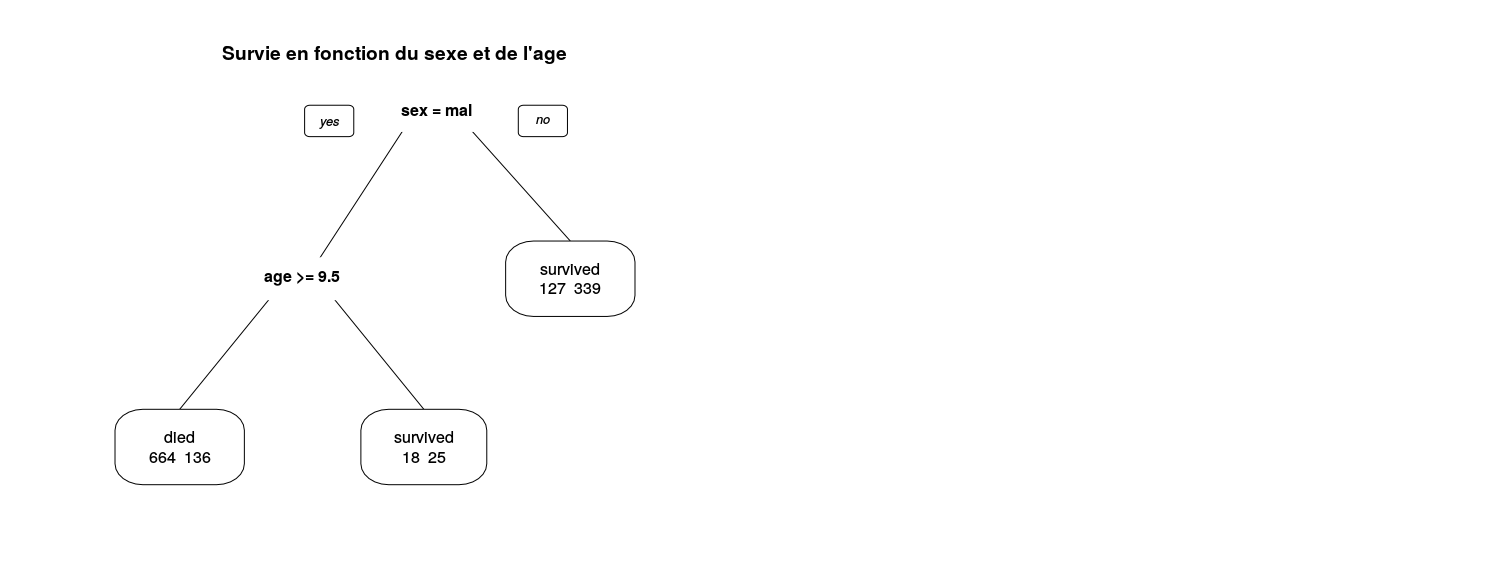
\includegraphics[width=\textwidth,height=0.8\textheight,keepaspectratio]{survie-sexe-age-base.png}
        \end{center}
\end{frame}

\begin{frame}
Nous avons les mêmes informations ici, cependant nous savons maintenant le pourcentage de personnes mortes et vivantes au lieu de leur nombre ainsi que le pourcentage
total de personnes que ce noeud représente par rapport au nombre total.
       \begin{center}
            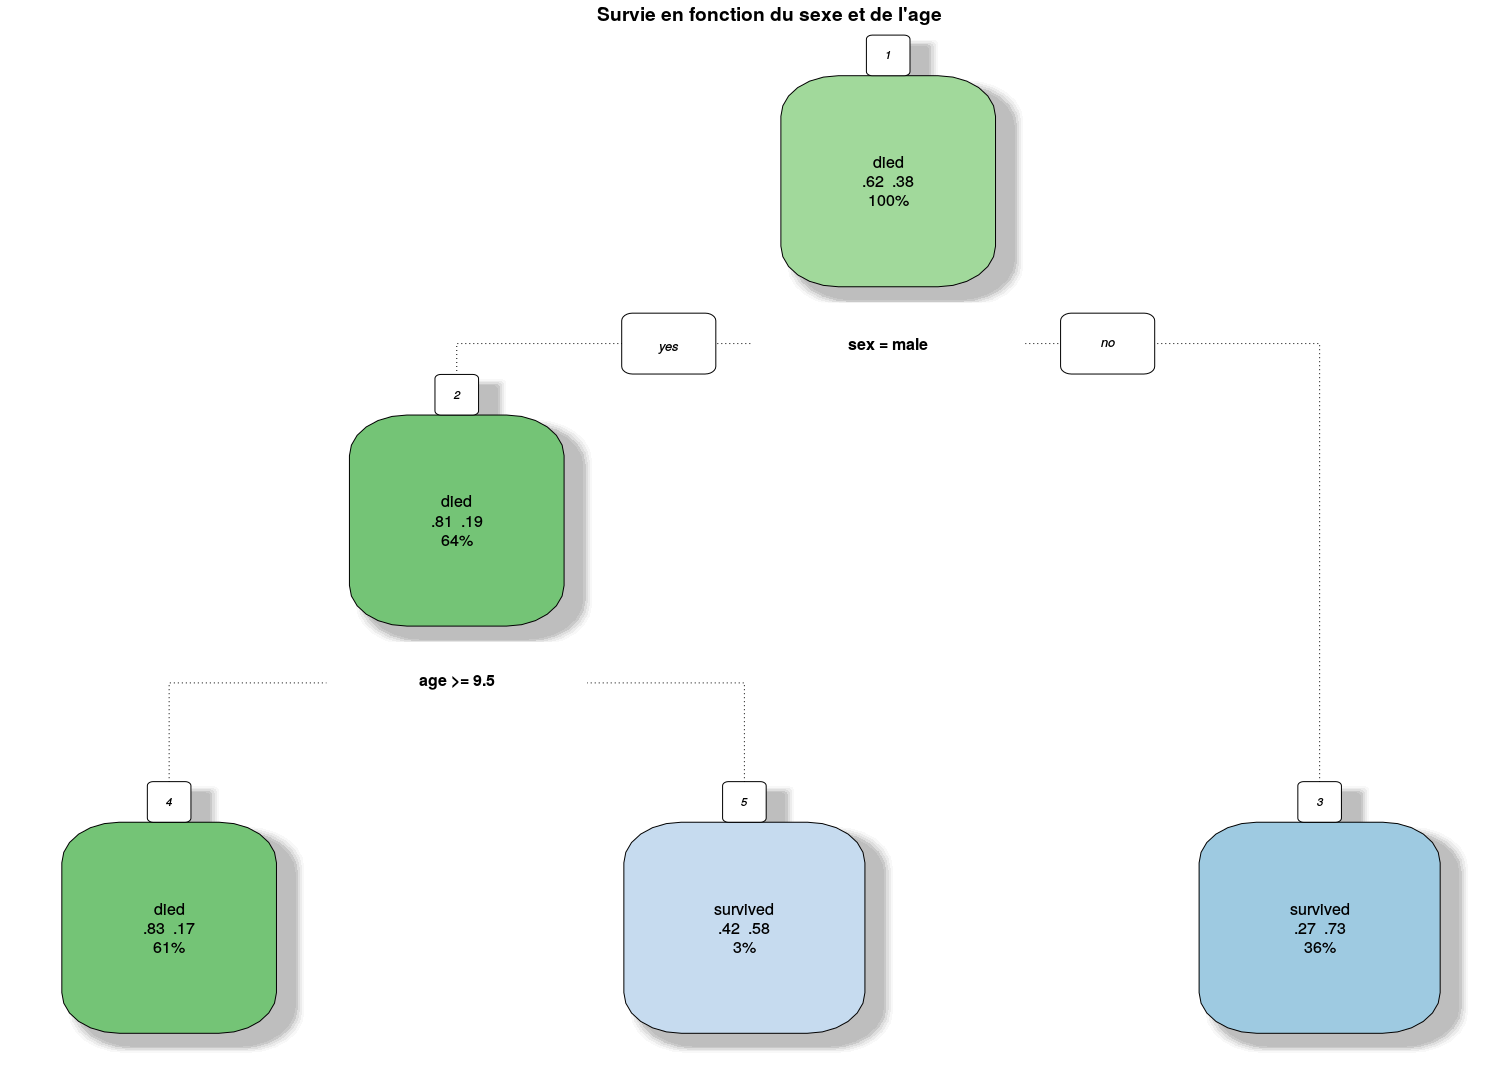
\includegraphics[width=\textwidth,height=0.8\textheight,keepaspectratio]{survie-sexe-age.png}
        \end{center}
\end{frame}


\begin{frame}
Le choix de la survie d'une personne se fait par rapport au pourcentage de personnes décédées par rapport aux surviants. 

 Nous allons montrer que cet arbre respecte l'algorithme de création décrit précédemment. Pour la survie en fonction de l'age et du sexe, l'arbre va devoir décider quel
 critère prendre en premier pour la séparation. Le meilleure critère est celui avec la meilleure différence de pureté. Comme calculé précédemment c'est
 le sexe qui permettra une meilleure séparation des données. L'abre respecte bien cette mesure

\end{frame}

\begin{frame}
 Voici comment améliorer l'arbre
\end{frame}

\begin{frame}
 Voici comment utiliser pour des valeurs non booléenne.
\end{frame}



\begin{frame}
 Nous allons maintenant montrer comment utiliser l'arbre construit via les données d'apprentissage pour prédire la valeur d'une des variable en fonction des autres.
 Nous allons utiliser des personnes pour lesquelles nous connaissons l'age, le sexe, la classe et le nombre de membres de la famille dans le bateau et nous prédirons
 si cette personne a survécu ou non en parcourant l'arbre. Le code suivant permet de faire cela :\\
 \lstinputlisting{predict.r}
 Nous prédisons ainsi le sort des 10 premiers passagers et le comparons aux valeurs théoriques obtenues. Nous remarquons que l'arbre a prédit correctement le sort
 de neuf de huit des dix passagers.
\end{frame}


\end{document}